\section{Trigger}\label{sec:Zprime_trigger}
The primary high level trigger (HLT) used in main analysis for 2016 and 2017 is HLT\_DoubleEle33\_CaloIdL\_MW which requires two electron candidates with $E_{T}$ of the supercluster higher than 33 GeV and passing loose calorimeter identification (CaloIdL) requirements and Medium Window (MW) matching between the gaussian sum filter (gsf) \cite{0954-3899-31-9-N01} track and the hits in pixel detector. In the run period of 276453 to 278822 of 2016 this trigger was prescaled and HLT\_DoubleEle33\_CaloIdL\_GsfTrkIdVL was used as the primary signal trigger. The HLT\_DoubleEle33\_CaloIdL\_GsfTrkIdVL is the same as HLT\_DoubleEle33\_CaloIdL\_MW except replacing MW pixel matching by very loose matching between gsf track and the supercluster in ECAL (GsfTrkIdVL).

The level 1 trigger (L1) seeding of the primary high level trigger is always seeded by the OR of a DoubleEG (two deposit in ECAL) seed, a SingleEG (one deposit in ECAL) seed and a SingleJet (one L1 object compatible with a jet) seed, after run 275319 in 2016 and in full 2017 it is also seeded by a SingleTau (one L1 object compatible with a $\tau$) seed. The presence of the SingleJet and SingleTau seeds are mean to mitigate the loss of efficiency for high $E_{T}$ electron. The exact unprescaled threshold of each of those seeds changing in time. The lowest threshold for the SingleEG which was always unprescaled was 40 GeV with the corresponding thresholds for the DoubleEG seed being 24 GeV,17 GeV.

The trigger efficiency will be split in L1 trigger efficiency, HLT supercluster $E_{T}$ filter efficiency (the HLT turn on curve) and online electron identification (CaloIdL+MW or GsfTrkIdVL) efficiency components. For final result only $E_{T}$ dependent efficiency will be used to weight MC events, others will be cancel in the normalisation of MC events to data in the Z peak region ($M_{ee}$ in 60-120 GeV). The method to measure the efficiency will be described in Section \ref{sec:trigger_efficiency_method}. The L1 trigger efficiency of primary signal trigger will be shown in Section \ref{sec:L1_trigger_efficiency}. The HLT $E_{T}$ turn on curve and HLT identification efficiency of primary signal trigger will be shown in Section \ref{sec:HLT_efficiency}, Other trigger efficiencies will be shown in Section \ref{sec:Other_HLT_efficiency}.

\subsection{Method for Measuring Trigger Efficiencies in Data}\label{sec:trigger_efficiency_method}
The tag and probe method \cite{CMS-AN-2009-111} is used to measure the efficiency in data. The event is selected by HLT\_Ele27\_eta2p1\_WPTight (require one HLT electron candidate with supercluster $E_{T}$ higher than 27 GeV and $|\eta|$ less than 2.1 and passing tight online electron cut) for 2016 and HLT\_Ele35\_WPTight (require one HLT electron candidate with supercluster $E_{T}$ higher than 35 GeV and passing tight online electron cut) for 2017. The tag is the electron which passing HLT\_Ele27\_eta2p1\_WPTight (HLT\_Ele35\_WPTight) in 2016 (2017) and passing HEEP ID (as defined in Section \ref{sec:Zprime_HEEP}) and in barrel of ECAL. The probe is the electron which passing the HEEP ID as well as any other requirements necessary to measure the given efficiency such as being matched to the $E_{T}$ filter to measure the trigger identification efficiency.

To simplify the computation, tags can not be probes. In the case of the probe being in the barrel, the tag is required to have a smaller supercluster $\phi$ than the probe for even number events and a larger supercluster $\phi$ for odd number events. As the sample is already very pure given there are two electrons passing HEEP ID, no background subtraction is applied, nor any mass window cut imposed. When measuring efficiencies involving the unseeded leg of the HLT\_DoubleEle33\_CaloIdL\_MW (or HLT\_DoubleEle33\_CaloIdL\_GsfTrkIdVL) trigger path, the tag should additionally pass the L1 seeded leg of that trigger and be matched to a L1 EG object, using a $\Delta R$ cone of 0.1 to be completely sure that the unseeded leg is unbiased by L1 seeded trigger. The efficiency is equal to the number of passing probes divided by all probes shown in \ref{eq:tag_probe_eff}.
\begin{equation}
\epsilon=\frac{N_{passing~probes}}{N_{all~probes}}
\label{eq:tag_probe_eff}
\end{equation}

The L1 trigger efficiency and HLT turn on curves are fitted with either a single or double turn on function (defined in terms of 'error function' $erf$). The double turn on function is shown in equation \ref{eq:turn_on}, with the single turn on function being identical except that the B terms are removed. The A0 and B0 parameters can be interpreted as the efficiency at the plateau, the A1 and B1 as the value where the efficiency reaches half maximum and A2 and B2 are the turn on of the curve.
\begin{equation}
f(E_{T})=0.5\cdot A0\cdot(1+erf(\frac{E_{T}-A1}{\sqrt{2}\cdot A2}))+0.5\cdot B0\cdot(1+erf(\frac{E_{T}-B1}{\sqrt{2}\cdot B2}))
\label{eq:turn_on}
\end{equation}

\subsection{Primary Signal Trigger: L1 Efficiency}\label{sec:L1_trigger_efficiency}
In 2016 the efficiency for a HEEP electron to pass the lowest unprescaled L1 SingleEG seed is shown in Figure \ref{fig:L1_eff_2016}. From applying to MC events, this translates to an efficiency of 99.5\% to select barrel-barrel and 98.8\% to select barrel-endcap events in a mass range of 60 to 120 GeV and a $\sim$100\% efficiency above 120 GeV. This is a lower bound on the efficiency, because there is the DoubleEG L1 seed which will further increase the efficiency. So it can be assumed the L1 seed trigger efficiency is 100\% with a 0.5\% uncertainty in the barrel and 1.2\% in the endcap.
\begin{figure}[h!]
\begin{center}
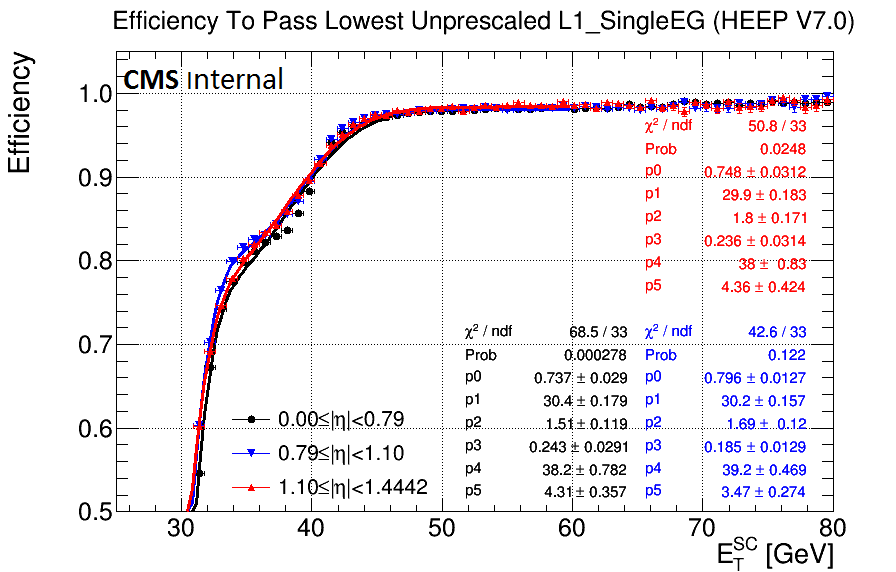
\includegraphics[width=0.45\textwidth]{figures/Zprime/2016/trigger/l1SingleEGEffEB.png}
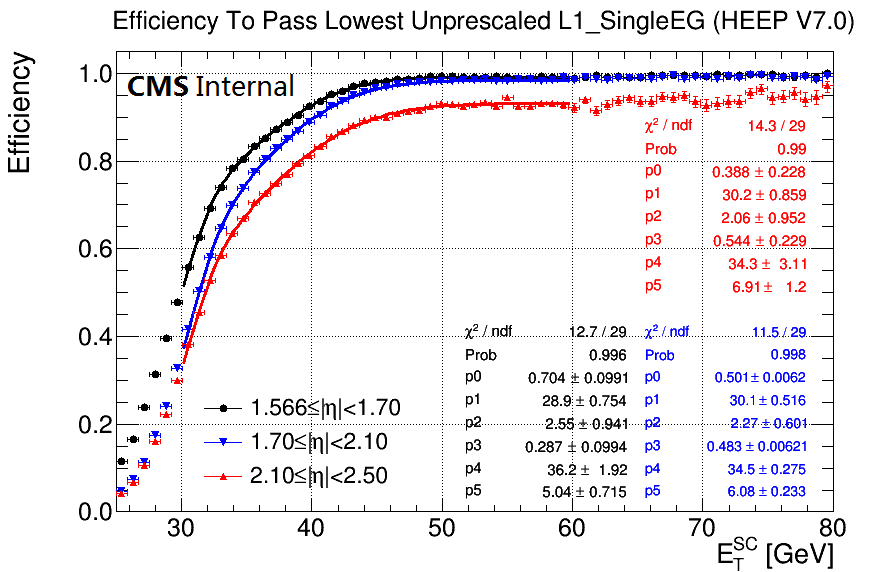
\includegraphics[width=0.45\textwidth]{figures/Zprime/2016/trigger/l1SingleEGEffEE.png}
\caption{The efficiency for an electron passing HEEP to pass the lowest unprescaled L1 SingleEG seed versus supercluster $E_{T}$ and $\eta$ in barrel (left) and in endcap (right) for 2016 \cite{CMS-AN-2016-404}.}
\label{fig:L1_eff_2016}
\end{center}
\end{figure}

In 2017 the efficiency for a HEEP electron to pass the lowest unprescaled L1 SingleEG seed is shown in Figure \ref{fig:L1_eff_2017}. In both barrel and endcap, a slow threshold related turn on and a slow general increase in efficiency in the plateau due to increasing efficiency of the L1 ID requirements are observed. From applying to MC events, this translates to an efficiency of 71\% to select barrel-barrel and 67\% to select barrel-endcap events with the worst case where the supercluster $E_{T}$ of both electrons is 35 GeV. The efficiency is higher than 99.5\% for two electrons with supercluster $E_{T}$ more than 42 GeV in barrel and more than 47 GeV in endcap. This is a lower bound on the efficiency, becasue there is the DoubleEG L1 seed which will further increase the efficiency.
\begin{figure}[h!]
\begin{center}
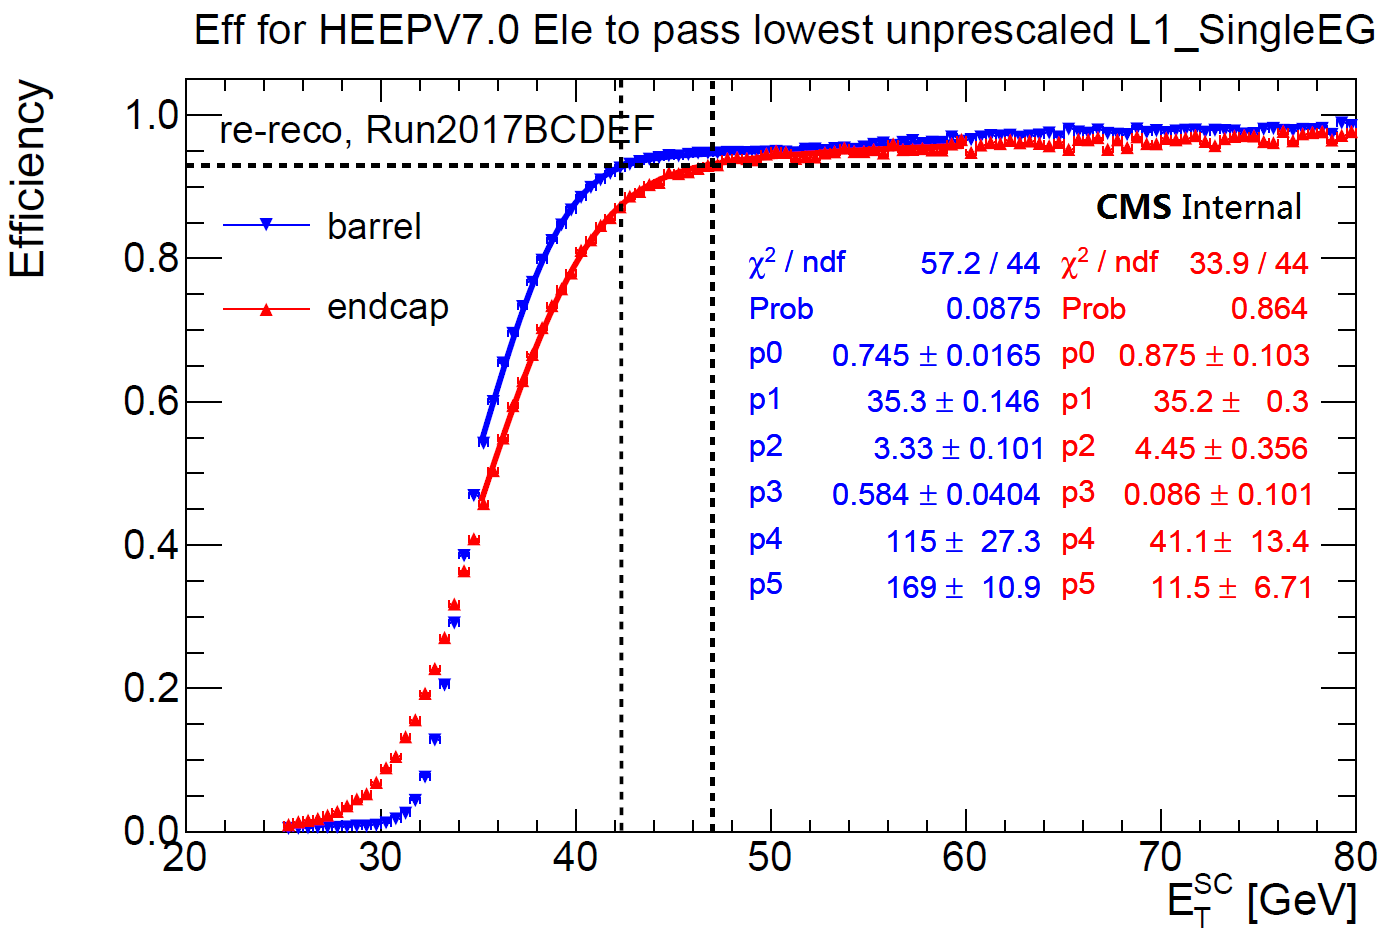
\includegraphics[width=0.5\textwidth]{figures/Zprime/2017/trigger/l1SingleEGEff.png}
\caption{The efficiency for an electron passing HEEP to pass the lowest unprescaled L1 SingleEG seed versus supercluster $E_{T}$ and $\eta$ in barrel and endcap for 2017 \cite{CMS-AN-2018-021}.}
\label{fig:L1_eff_2017}
\end{center}
\end{figure}

Due to the fact that the L1 efficiency is not 100\% for low $E_{T}$ electrons in 2017, the L1 seeded trigger turn on is considered in the 2017 analysis as described below. In data, we require for at least one of the selected electrons to be matched with the object of L1 seed trigger filter of the HLT\_DoubleEle33\_CaloIdL\_MW and with that object having a L1 $E_{T}$ greater than the lowest unprescaled L1 SingleEG seed $E_{T}$ threshold. Therefore, only L1 SingleEG seed turn on shown in Figure \ref{fig:L1_eff_2017} is used to weight MC events. Since only one electron is seeded by L1 in HLT\_DoubleEle33\_CaloIdL\_MW, the L1 weight value of selected MC events are shown in equation \ref{eq:L1_turn_on} where $P_{1}$ and $P_{2}$ are the L1 SingleEG efficiencies (shown in Figure \ref{fig:L1_eff_2017}) for leading and sub-leading selected HEEP electrons.
\begin{equation}
weight(L1)=1-(1-P_{1})\cdot(1-P_{2})=P_{1}+P_{2}-P_{1}P_{2}
\label{eq:L1_turn_on}
\end{equation}


\subsection{Primary Signal Trigger:HLT Efficiency}\label{sec:HLT_efficiency}
The HLT efficiency is divided into two components, the efficiency of the supercluster $E_{T}>33$ GeV cut (the turn on curve) and the efficiency of the CaloIdL plus MW matching (or GsfTrkIdVL) identification requirements. The turn on curves of the $E_{T}$ cut for 2016 and 2017 are shown in Figure \ref{fig:HLT_turnon_2016} and Figure \ref{fig:HLT_turnon_2017} respectively. These turn on curves are used to weight the MC events.
The efficiency of the CaloIdL plus MW matching (or GsfTrkIdVL) identification requirements for 2016 and 2017 are shown in Figure \ref{fig:HLT_ID_2016} and Figure \ref{fig:HLT_ID_2017} respectively. As the efficiencies are flat versus $E_{T}$, there is no need to weight MC events with this factor as it will automatically be included in the Z peak normalisation.

\begin{figure}[h!]
\begin{center}
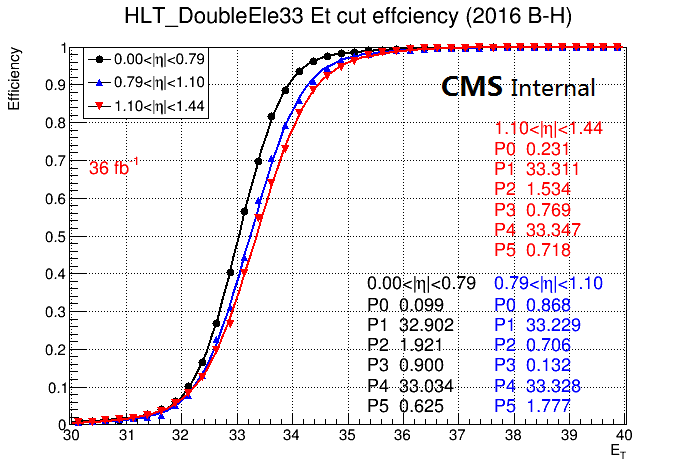
\includegraphics[width=0.45\textwidth]{figures/Zprime/2016/trigger/turnOnEEUnseeded.png}
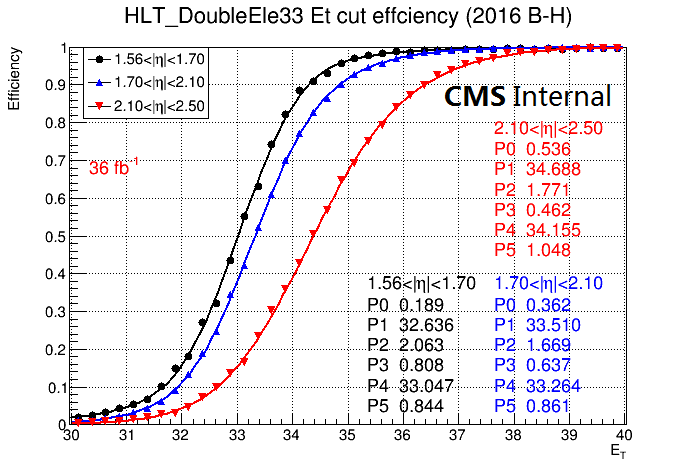
\includegraphics[width=0.45\textwidth]{figures/Zprime/2016/trigger/turnOnEBUnseeded.png}
\caption{The efficiency for electron in the barrel (left) and endcap (right) passing HEEP to pass an online supercluster $E_{T}$ > 33 GeV cut for 2016 \cite{CMS-AN-2016-404}.}
\label{fig:HLT_turnon_2016}
\end{center}
\end{figure}

\begin{figure}[h!]
\begin{center}
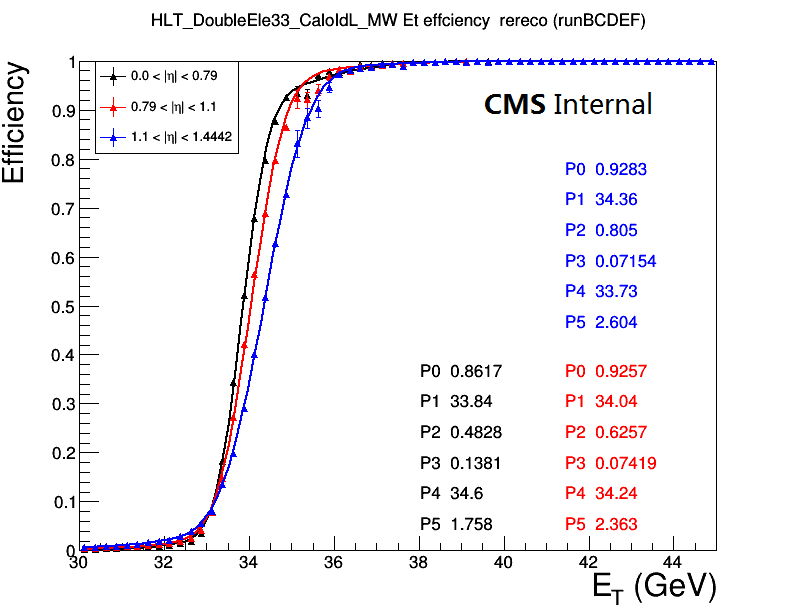
\includegraphics[width=0.45\textwidth]{figures/Zprime/2017/trigger/eff_DouEle33_Et_barrel.png}
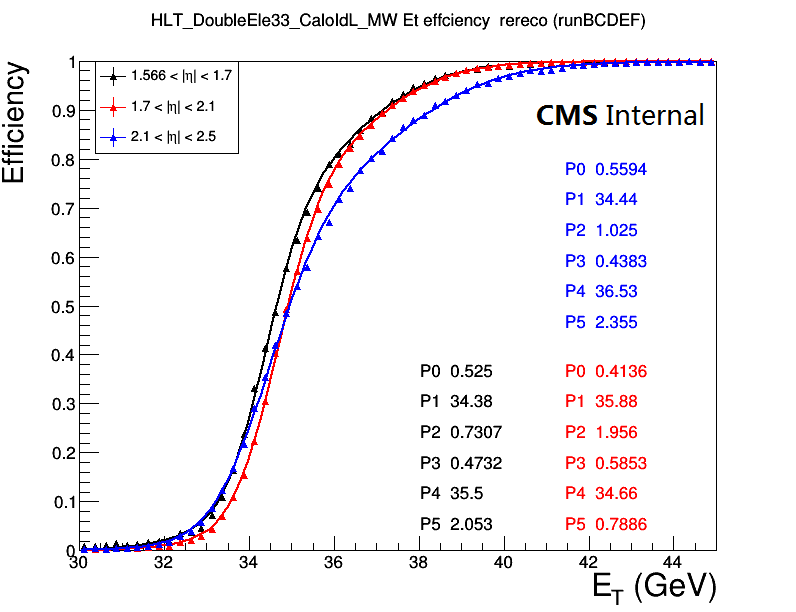
\includegraphics[width=0.45\textwidth]{figures/Zprime/2017/trigger/eff_DouEle33_Et_endcap.png}
\caption{The efficiency for electron in the barrel (left) and endcap (right) passing HEEP to pass an online supercluster $E_{T}$ > 33 GeV cut for 2017 \cite{CMS-AN-2018-021}.}
\label{fig:HLT_turnon_2017}
\end{center}
\end{figure}

\begin{figure}[h!]
\begin{center}
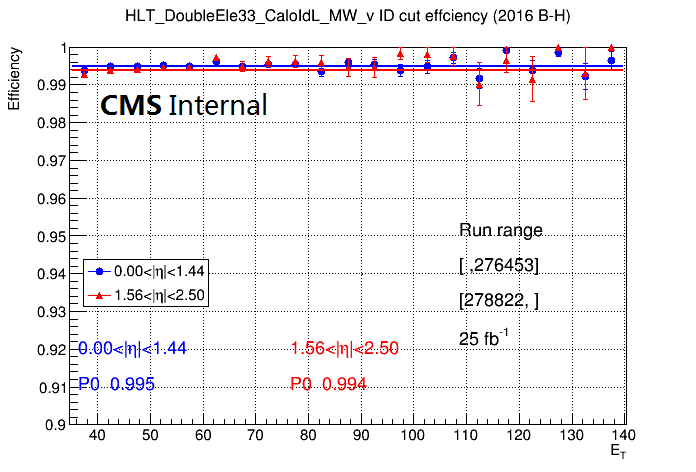
\includegraphics[width=0.45\textwidth]{figures/Zprime/2016/trigger/effMW1_DoubleEle33_SingleElectron_ID_matchedMethod.png}
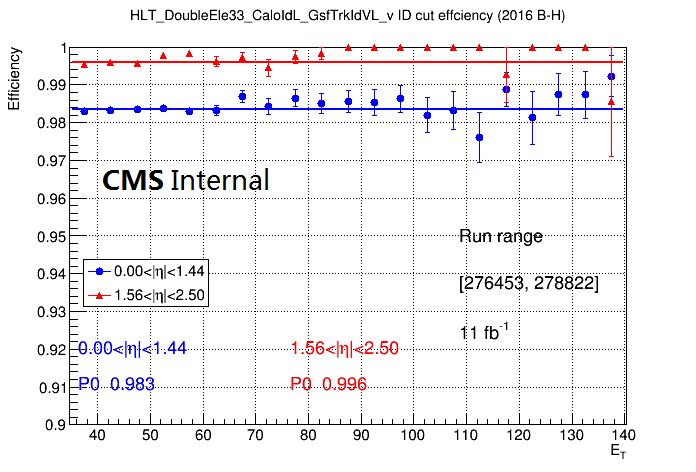
\includegraphics[width=0.45\textwidth]{figures/Zprime/2016/trigger/eff1_DoubleEle33_SingleElectron_ID_matchedMethod.png}
\caption{The efficiency for electron in the barrel and endcaps passing HEEP to pass the CaloIdL+MW ID requirement(left) and CaloIdL+GsfTrkIdVL ID requirement (right) for 2016 \cite{CMS-AN-2016-404}.}
\label{fig:HLT_ID_2016}
\end{center}
\end{figure}

\begin{figure}[h!]
\begin{center}
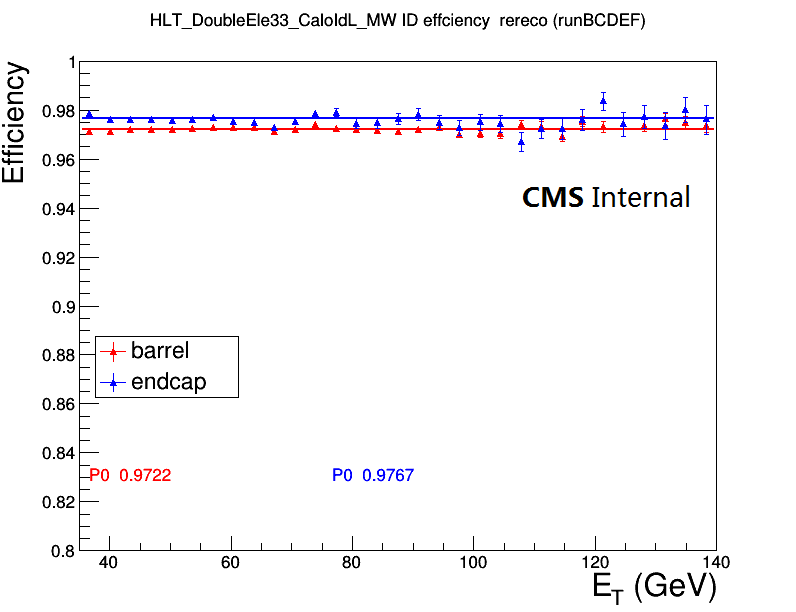
\includegraphics[width=0.5\textwidth]{figures/Zprime/2017/trigger/eff_DouEle33_ID.png}
\caption{The efficiency for electron in the barrel and endcaps passing HEEP to pass the CaloIdL+MW ID requirement for 2017 \cite{CMS-AN-2018-021}.}
\label{fig:HLT_ID_2017}
\end{center}
\end{figure}

\subsection{Other Trigger Efficiencies}\label{sec:Other_HLT_efficiency}
In 2016 the data-MC HEEP ID efficiency scale factor study uses events selected by the \\
HLT\_Ele27\_eta2p1\_WPTight trigger path. The efficiency of this path in data is shown in Figure \ref{fig:Ele27_2016}. Similar for 2017 the HLT\_Ele35\_WPTight trigger path is used and the efficiency of this trigger is shown in Figure \ref{fig:Ele35_2017}. These curves are used to weight MC events to simulate the effect of the trigger requirement in data.

\begin{figure}[h!]
\begin{center}
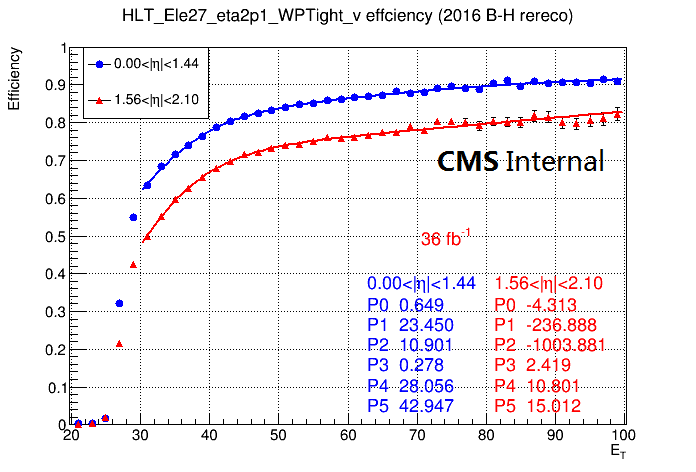
\includegraphics[width=0.5\textwidth]{figures/Zprime/2016/trigger/ele27Eff.png}
\caption{The efficiency for an electron passing HEEP to pass the HLT\_Ele27\_eta2p1\_WPTight trigger for 2016 \cite{CMS-AN-2016-404}.}
\label{fig:Ele27_2016}
\end{center}
\end{figure}

\begin{figure}[h!]
\begin{center}
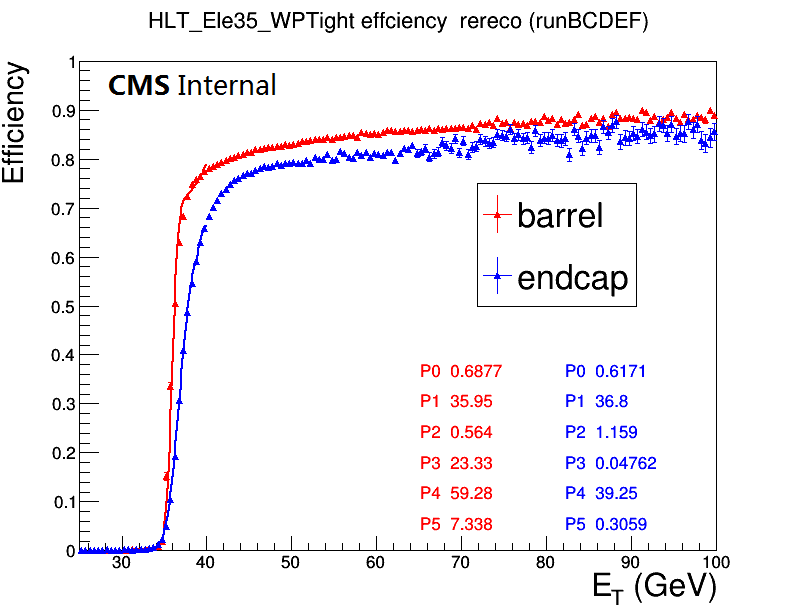
\includegraphics[width=0.45\textwidth]{figures/Zprime/2017/trigger/eff_Ele35_part1.png}
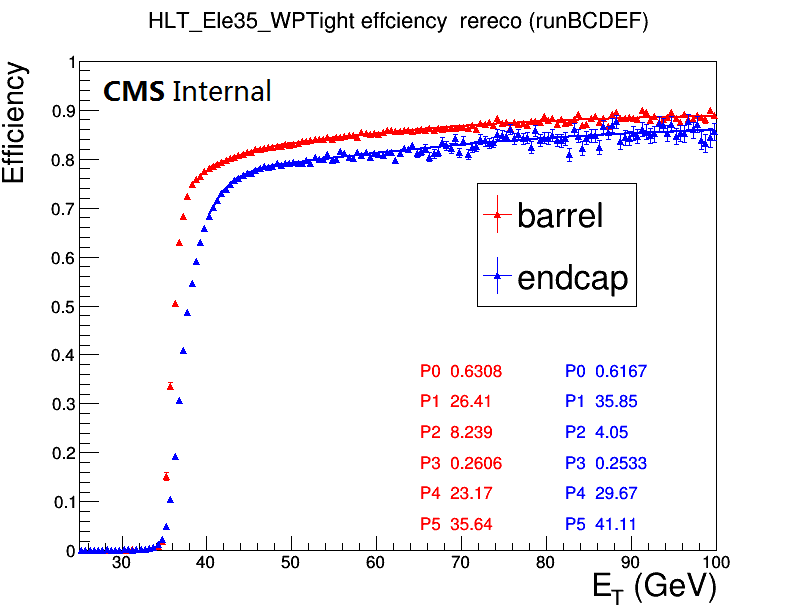
\includegraphics[width=0.45\textwidth]{figures/Zprime/2017/trigger/eff_Ele35_part2.png}
\caption{The efficiency for an electron passing HEEP to pass the HLT\_Ele35\_WPTight for $E_{T}$ less than 40 GeV (left) and $E_{T}$ more than 40 GeV (right) for 2017 \cite{CMS-AN-2018-021}.}
\label{fig:Ele35_2017}
\end{center}
\end{figure}
